\chapter{Analysis Optimization}\label{sec:analysis_optimization}
\red{add mjj etajj input vars}
After selecting objects that represent the final state of the physical process under investigation, a metric needs to be constructed sensitive to the outcomes of a hypothesis test. Often, this metric takes the form of a kinematic variable, such as the invariant mass of the Higgs pair system $m_\text{HH}$ in this analysis, designed to differentiate between signal and background events. As elaborated in Chapter \ref{sec:statistics}, the underlying statistical test employs frequentist principles, thus histograms derived from this metric serve as inputs to these tests. Throughout the development of this variable, various optimizations typically aim to maximize the signal-to-background ratio as a proxy for the statistical tests expressivity. This ratio

Since the purpose of this quantity is to separate signal from background it is well suited to be anaylized with a \ac{ml} model. While such models have gained widespread usage in particle physics \citep{albertsson2019machine,shlomi2020graph,feickert2021living,Schwartz2021Modern}, their effectiveness is limited when they are only optimized for signal-to-background discrimination. This is because their training does not usually consider broader goals like assessing discovery significance or establishing confidence levels.

The signal-to-background ratio or the efficacy of a \ac{ml} model in separating events correlates to some extent with the performance of the statistical test. However, this relationship often remains suboptimal because uncertainties, which can significantly influence the outcome of hypothesis tests, are not typically considered during the training phase of \ac{ml} models.

To address these challenges, \textit{\ac{neos}} \citep{Simpson_2023} offers a promising solution. This approach incorporates the statistical model and its uncertainties into the \ac{ml} model's training process, aligning it more closely with the primary goal of determining whether a new process exists. This chapter introduces machine learning concepts and elaborates on the \textit{\ac{neos}} methodology and its implementation in this analysis with the \ac{tomatos} training framework.

% To overcome these limitations, the \textit{\ac{neos}} approach \citep{Simpson_2023} presents a valuable strategy. It integrates the statistical model and its associated uncertainties directly into the \ac{ml} model training, thereby aligning the model more closely with the fundamental objective of confirming the existence of new processes. This chapter introduces machine learning concepts and elaborates on the \textit{\ac{neos}} methodology and its implementation in this analysis.
% To address these challenges, \textit{\ac{neos}} \citep{Simpson_2023} offers a promising solution. This approach incorporates the statistical model and its uncertainties into the \ac{ml} model's training process, aligning it more closely with the primary goal of determining whether a new process exists. This chapter provides a brief introduction to machine learning and explains the \textit{\ac{neos}} approach and its application in this analysis in detail.

\section{Machine Learning}
\ac{ml} refers to algorithms that enable computers to learn from data to make predictions for some specific task without being explicitly programmed for \citep{kubat2021introduction}. One particular subset of \ac{ml} models are \acp{ann} inspired by the human brain. Their fundamental unit are nodes, the neurons, that are interconnected to other neurons. If they organized in consecutive layers with an initial input and a desired output as shown in figure \ref{fig:ann} they are referred to deep feed-forward \acp{nn}. The signals between neurons are transferred weighted and each neuron has an activation function that converts the received input stimulus into an output strength. Thus learning occurs through adjusting the weights between the neurons. \acp{ann} can be designed in various ways with many layers depending on the specific task.
\begin{figure}
    \centering
    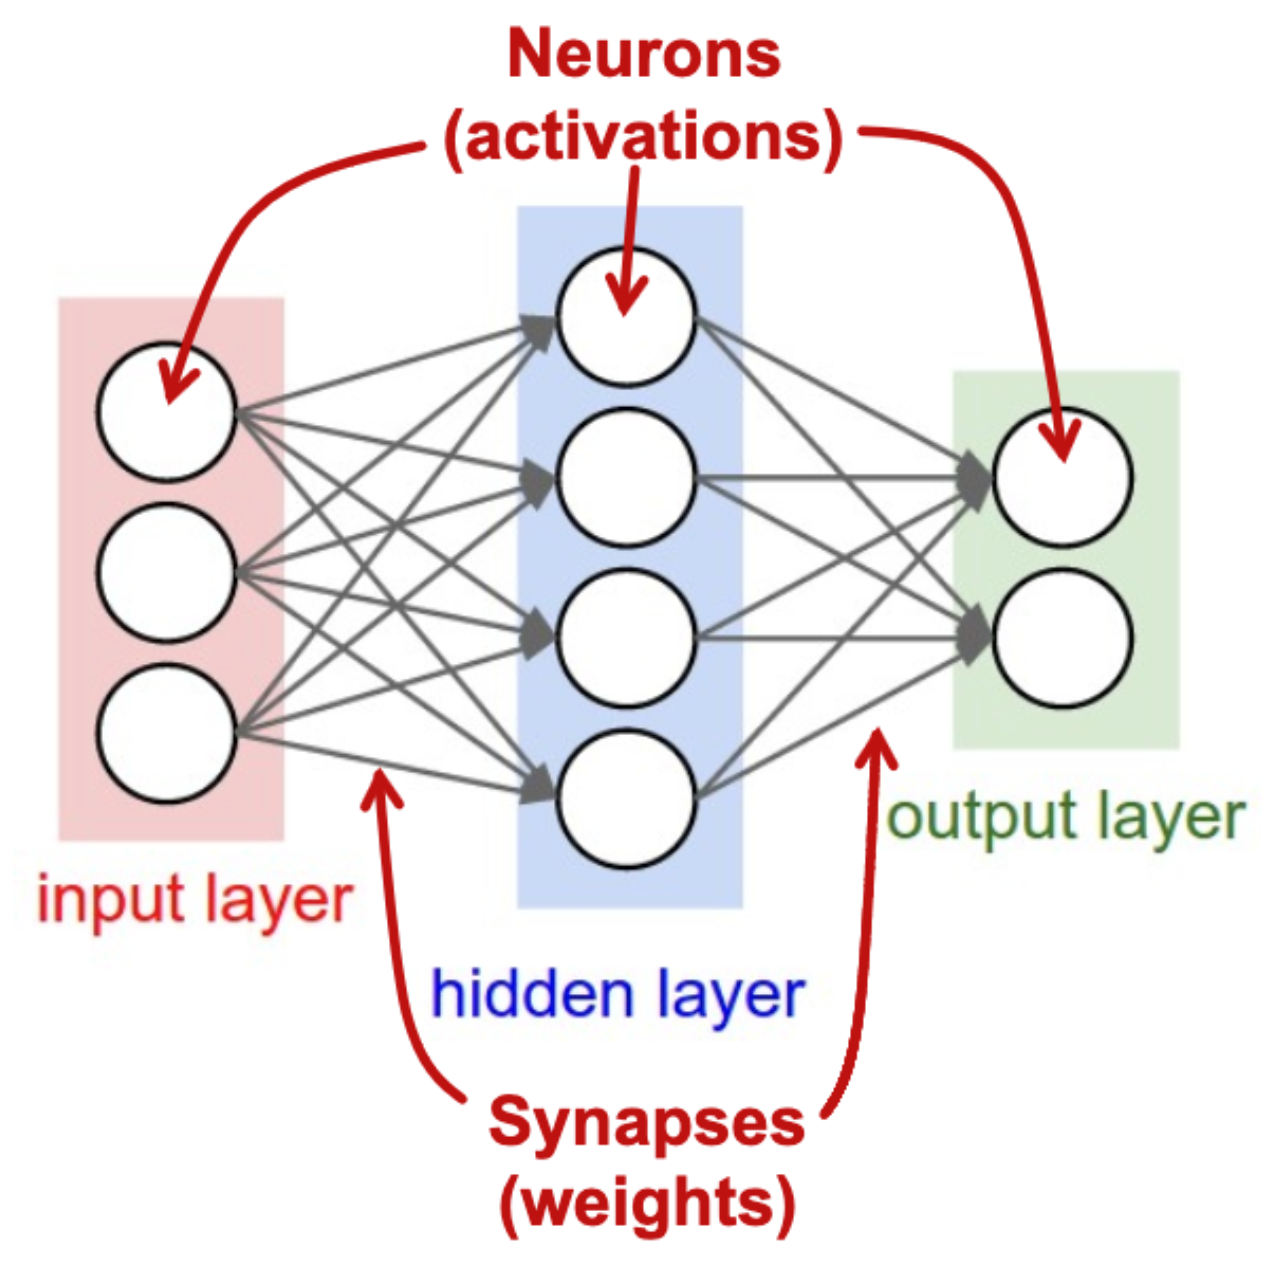
\includegraphics[width=0.4\textwidth]{ann}
    \caption[]{Structure of artificial feed-forward neural networks. Adopted from \citep{8114708}.}
    \label{fig:ann}
\end{figure}

The training of \acp{nn} is usually performed with the back-propagation algorithm which seeks to minimize a cost function $C(\bm{\varphi})$. This function measures the deviation of a given input from a desired output as a function of the model parameters $\bm{\varphi}$. For training a binary classifier, where the output ranges continuously from 0 to 1, e.g. 1 indicating signal and 0 indicating background, the \ac{bce} cost function is widely used:
\begin{equation}\label{eq
    }
    C = -\frac{1}{N} \sum_{i=1}^{N} \left[ y_i \log(p_i) + (1 - y_i) \log(1 - p_i) \right],
\end{equation}
where $N$ is the total number of training examples, $y_i$ represents the true label and $p_i$ the predicted value by the \ac{nn} of the $i$-th training example.

In a deep feed-forward \ac{nn} these model parameters are the mentioned weights and a bias term added to the sum of the input weights per neuron. The minimum of this cost function can be found stepwise via gradient descent. Here, the update to the model parameters is guided by the negative of the gradient of the cost function, scaled by a learning rate $\gamma$
\begin{equation}
    \bm{\varphi}_{n+1} = \bm{\varphi}_n-\gamma\nabla C(\bm{\varphi}_n),
    \label{eq:grad_descent}
\end{equation}
such that moving against the gradient a monotonic decreasing series is formed $C(\bm{\varphi}_n )\ge C(\bm{\varphi}_{n+1})$ converging to a minimum of $C(\bm{\varphi})$. In three dimensions this is analogues to a mountaineer searching for the valley by going in the direction of the steepest descent with a stepsize proportional to $\gamma$.

\section{NEOS}
The core innovation of \textit{\ac{neos}} lies in integrating the final quantity of interest into the training process. Rather than employing a traditional \ac{bce} cost function from equation \ref{eq:bce} focused solely on distinguishing between signal and background, the $\mathrm{CL}s$ value, detailed in Chapter \ref{sec:statistics}, is adopted as the quantity for minimization. As depicted in Figure \ref{fig:neos}, this approach effectively results in a mathematical concatenation of the individual steps within the typical analysis chain.

\begin{figure}
    \centering
    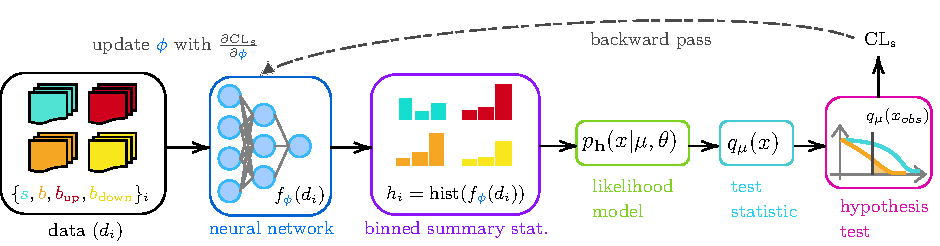
\includegraphics[width=1\textwidth]{neos}
    \caption[]{Typical particle physics analysis chain. For \ac{neos} the $\text{CL}_s$ value is back-propagated to train the neural network parameters $\bm{\varphi}$. Adopted from \citep{Simpson_2023}.}
    \label{fig:neos}
\end{figure}
Hence the cost function $\text{CL}_s$ is a function of the dataset $\mathcal{D}$ and the \ac{ml} model parameters $\bm{\varphi}$
\begin{equation}
    \mathrm{CL}_s = f(\mathcal{D},\bm{\varphi}) = (f_{\mathrm{sensitivity}} \circ f_{\mathrm{test\,stat}} \circ f_{\mathrm{likelihood}}  \circ f_{\mathrm{histogram}}  \circ f_{\mathrm{observable}})(\mathcal{D},\bm{\varphi}).
\end{equation}
In order to find the minimum via the gradient descent of equation \ref{eq:grad_descent} \cls needs to be differentiable with respect to $\bm{\varphi}$. By applying the chain rule this reads for one model parameter $\varphi_i$
\begin{equation}
    \frac{\partial\,\mathrm{CL}_s}{\partial \varphi_i} = \frac{\partial f_{\mathrm{sensitivity}}}{\partial f_{\mathrm{test\,stat}}}\frac{\partial f_{\mathrm{test\,stat}}}{\partial f_{ \mathrm{likelihood}}} \frac{\partial f_{\mathrm{likelihood}}}{\partial f_{\mathrm{histogram}}}   \frac{\partial f_{\mathrm{histogram}}}{\partial f_{\mathrm{observable}}}  \frac{\partial f_{\mathrm{observable}}}{\partial \varphi_i}.
\end{equation}
While all steps except histogramming are inherently differentiable, histogramming can be made differentiable through the application of \ac{kde}, as described by \citep{CRANMER2001198}. This technique involves approximating histograms by treating each data point as a normal distribution (kernel) centered at the data point value, with a bandwidth corresponding to the desired standard deviation. Since the area under each Gaussian is equal to one, the collective addition of all Gaussian's yields a smoothed estimate of a histogram that is inherently differentiable. However, it is crucial to select the bandwidth appropriately, ideally around the desired bin width, as the quality of the KDE estimate is sensitive to this choice. This is demonstrated in figure \ref{fig:relaxed_hist}. Although this can be a source of uncertainty any differentiable step or block in figure \ref{fig:neos} can always be reverted and calculated exactly after optimized parameters have been found.
\begin{figure}
    \centering
    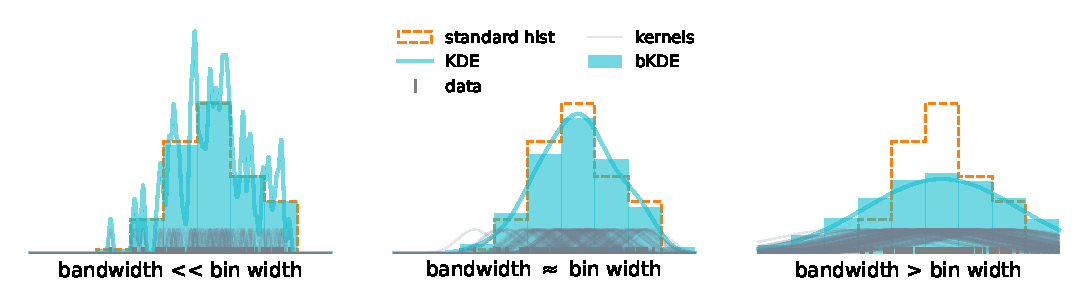
\includegraphics[width=1\textwidth]{relaxed_hist}
    \caption[]{Dependence of the histogram approximation with normal distributions of different standard deviations called bandwidth in the context of \ac{kde}. Depicted in grey small bars on the x-axis are the data points and in grey above them their kernel estimates. Further shown is the standard histogram binned from data, the \ac{kde} and the \ac{bkde} as a histogram calculated from the area under the \ac{kde} for some binning. Adopted from \citep{Simpson_2023}.}
    \label{fig:relaxed_hist}
\end{figure}



\subsection{Implementation}
Tracing differentiation through software is achievable by recognizing that any software essentially comprises a series of elementary arithmetic operations. Since the analytic solutions for these operations are known, the task reduces to concatenating all these operations and differentiating the resulting function. This is also known as \textit{Automatic Differentiation} and is achieved here with the help of the software package \textsc{jax} \citep{jax2018github} which also  integrates easily into \ac{ml} libraries.

While the concept may appear straightforward, one of the challenges that previously hindered its implementation is the difficulty of differentiating across multiple individual software frameworks used in the individual steps of figure \ref{fig:neos}. That this became feasible within a reasonable time frame builds greatly on some transition efforts to the \textsc{Python} programming language from C++ \textsc{root}-based software \citep{ANTCHEVA20092499} used in \ac{hep}. While \textsc{root} was indispensable at its time of emergence, Python offers significant advantages with its ease of use and extensive libraries and frameworks that work seamlessly together, which is essential for the required \ac{ml} techniques. Having all the steps in figure \ref{fig:neos} available as Python tools, has enabled the use of tools like \textsc{jax}, which are not originally connected to \ac{hep}.

The original proposers \citet{Simpson_2023} of \ac{neos} developed differentiable versions of common \ac{hep} tasks like the upper mentioned hypothesis test, histogramming and the optimization of a cut in a packaged called \textsc{relaxed} \citep{Simpson_relaxed_version_0_3_0_2023}. They successfully tested the entire pipeline in a toy model \citep{Simpson_neos_version_0_2_0_2021}. For this thesis these efforts were further developed within a framework called \textit{\acf{tomatos}} \citep{tomatos} and applied to an \ac{atlas} analysis. This included a code refactoring, data preprocessing, implementation of weighted histogramming, integration of an appropriate \ac{ml} library, and validation methods.


\section{Training}\label{sec:neos_training}
In order to build the statistical model each histogram entering it needs to be filled from data during the training. This requires a full dataset of variables per sample (signal, background estimate, systematic) being processed through the whole pipeline as of figure \ref{fig:neos}. The \ac{tomatos} \citep{tomatos} training framework encapsulates the following techniques.

\acp{nn} tend to learn from more frequently observed data. Thus to make use of all available data and to avoid a training class imbalance each sample is upscaled by replicating values to the sample with the largest event content, which in this case is a sample with the systematic: `JET EtaIntercalibration NonClosure PreRec up'. This is a result of a slightly increased selection efficiency if $\eta$ is varied upwards. To avoid artificially altering the event counts in the histograms, a scale factor of $n_\text{sample}/n_\text{max}$ is applied to the weights.

Table \ref{tab:neos-samples} gives an overview of used samples and the number of events they contain. Only uncertainties with an impact on an \mhh{} fit as of figure \ref{fig:m_hh_full_sys_ranking} are used to speed up the training process. These uncertainties are detailed in chapter \ref{sec:systematics} and comprise the 4 $b$-quark branching ratio normalization, the statistical error on the ABCD method transfer factor extraction and the shape uncertainty associated to this method, the four estimated $p_T$ binned uncertainties of the GN2X tagger, the envelope of the scale variations, the statistical errors on the \ktwov signal sample and the background estimate and two $\eta$ small-$R$ jet uncertainties. Table \ref{tab:neos-samples} also reveals that the background estimate is upscaled by a factor of $\sim 2$. Input variables per sample are shown in figure \ref{fig:tomatos_inputs_0} and \ref{fig:tomatos_inputs_1}. To ensure a fair training across features and prevent those with large values from dominating the learning process, a min-max scaling is applied to the inputs:
\begin{equation}
    x'=\frac{x - \text{min}(x)}{\text{max}(x)-\text{min}(x)},
\end{equation}
scaling them between 0 and 1. \qty[]{90}{\percent} of events in the dataset are used for training (39713 events), whereas the other \qty[]{10}{\percent} are again split into a \qty[]{80}{\percent} validation sample (3530 events) and \qty[]{20}{\percent} test sample (883 events). The epoch with the lowest loss value when evaluated on the validation sample is chosen after training.

In addition four samples are processed through the pipeline to estimate the background with the ABCD method described in \ref{sec:abcd}. The transfer factor and its uncertainty is estimated from the \ac{cr} and a shape uncertainty is estimated in the \ac{vr} as described in \ref{sec:bkg_uncertainties}. The downward uncertainty estimate is unbound such that it can assume negative values during optimization. This resulted in improved cross-section limits determined after optimization when the ucnertainty is bounded at zero. \red{need to redo with mix-max scale on alle samples, as currently clipped The Min-Max scaling for the input variables is derived on the \ac{sr} and thus only knows about mass values for the Higgs candidate for that region. } Event numbers are also shown in table \ref{tab:neos-samples}. Per training epoch, which corresponds to a full processing of the dataset, data are reshuffled.

The optimization also optimizes cuts on the invariant mass $m_{jj}$ and the pseudorapidity difference $|\Delta\eta(j,j)|$ of the two \ac{vbf} jets as mentioned in \ref{sec:hh4b_analysis_strategy}. Mathematically, applying a cut can be represented by multiplying the value to be cut with a Heaviside function shifted by the cut value. For a differentiable approximation, a sigmoid function is used, which is then multiplied to an event's weight.

\red{update table}
\begin{table}[]
    \centering
    \caption{Samples and available number of events after the selection described in section \ref{sec:hh4b_analysis_strategy} used in the training. Systematics are described in \ref{sec:systematics}. Deviations }
    \begin{tabular}{lr}
        \hline
        Sample (Systematic)                                                            & Events \\ \hline \hline
        Data Background Estimate                                                       & 21913  \\ \hline
        Signal $\kappa_\mathrm{2V}=0$ (Nominal)                                        & 43492  \\
        Signal $\kappa_\mathrm{2V}=0$ (GN2X pt bin 0 up)                               & 43492  \\
        Signal $\kappa_\mathrm{2V}=0$ (GN2X pt bin 0 down)                             & 43492  \\
        Signal $\kappa_\mathrm{2V}=0$ (GN2X pt bin 1 up)                               & 43492  \\
        Signal $\kappa_\mathrm{2V}=0$ (GN2X pt bin 1 down)                             & 43492  \\
        Signal $\kappa_\mathrm{2V}=0$ (GN2X pt bin 2 up)                               & 43492  \\
        Signal $\kappa_\mathrm{2V}=0$ (GN2X pt bin 2 down)                             & 43492  \\
        Signal $\kappa_\mathrm{2V}=0$ (GN2X pt bin 3 up)                               & 43492  \\
        Signal $\kappa_\mathrm{2V}=0$ (GN2X pt bin 3 down)                             & 43492  \\
        Signal $\kappa_\mathrm{2V}=0$ (JET EtaIntercalibration NonClosure PreRec up)   & 44126  \\
        Signal $\kappa_\mathrm{2V}=0$ (JET EtaIntercalibration NonClosure PreRec down) & 42737  \\
        Signal $\kappa_\mathrm{2V}=0$ (JET EtaIntercalibration Modelling up)           & 43917  \\
        Signal $\kappa_\mathrm{2V}=0$ (JET EtaIntercalibration Modelling down)         & 42984  \\
        Signal $\kappa_\mathrm{2V}=0$ (Scale Variation $\mu_R = 0.5, \mu_F=0.5)$       & 43492  \\
        Signal $\kappa_\mathrm{2V}=0$ (Scale Variation $\mu_R = 0.5, \mu_F=1.0)$       & 43492  \\
        Signal $\kappa_\mathrm{2V}=0$ (Scale Variation $\mu_R = 1.0, \mu_F=0.5)$       & 43492  \\
        Signal $\kappa_\mathrm{2V}=0$ (Scale Variation $\mu_R = 1.0, \mu_F=1.0)$       & 43492  \\
        Signal $\kappa_\mathrm{2V}=0$ (Scale Variation $\mu_R = 1.0, \mu_F=2.0)$       & 43492  \\
        Signal $\kappa_\mathrm{2V}=0$ (Scale Variation $\mu_R = 2.0, \mu_F=1.0)$       & 43492  \\
        Signal $\kappa_\mathrm{2V}=0$ (Scale Variation $\mu_R = 2.0, \mu_F=2.0$)       & 43492  \\ \hline
        Signal $\kappa_\mathrm{2V}=0$ (\ac{cr}, GN2X tags: 1)                          & 142443 \\
        Signal $\kappa_\mathrm{2V}=0$ (\ac{cr}, GN2X tags: 2)                          & 544    \\
        Signal $\kappa_\mathrm{2V}=0$ (\ac{vr}, GN2X tags: 1)                          & 57098  \\
        Signal $\kappa_\mathrm{2V}=0$ (\ac{vr}, GN2X tags: 2)                          & 243    \\
    \end{tabular}
    \label{tab:neos-samples}
\end{table}


\begin{figure}
    \centering
    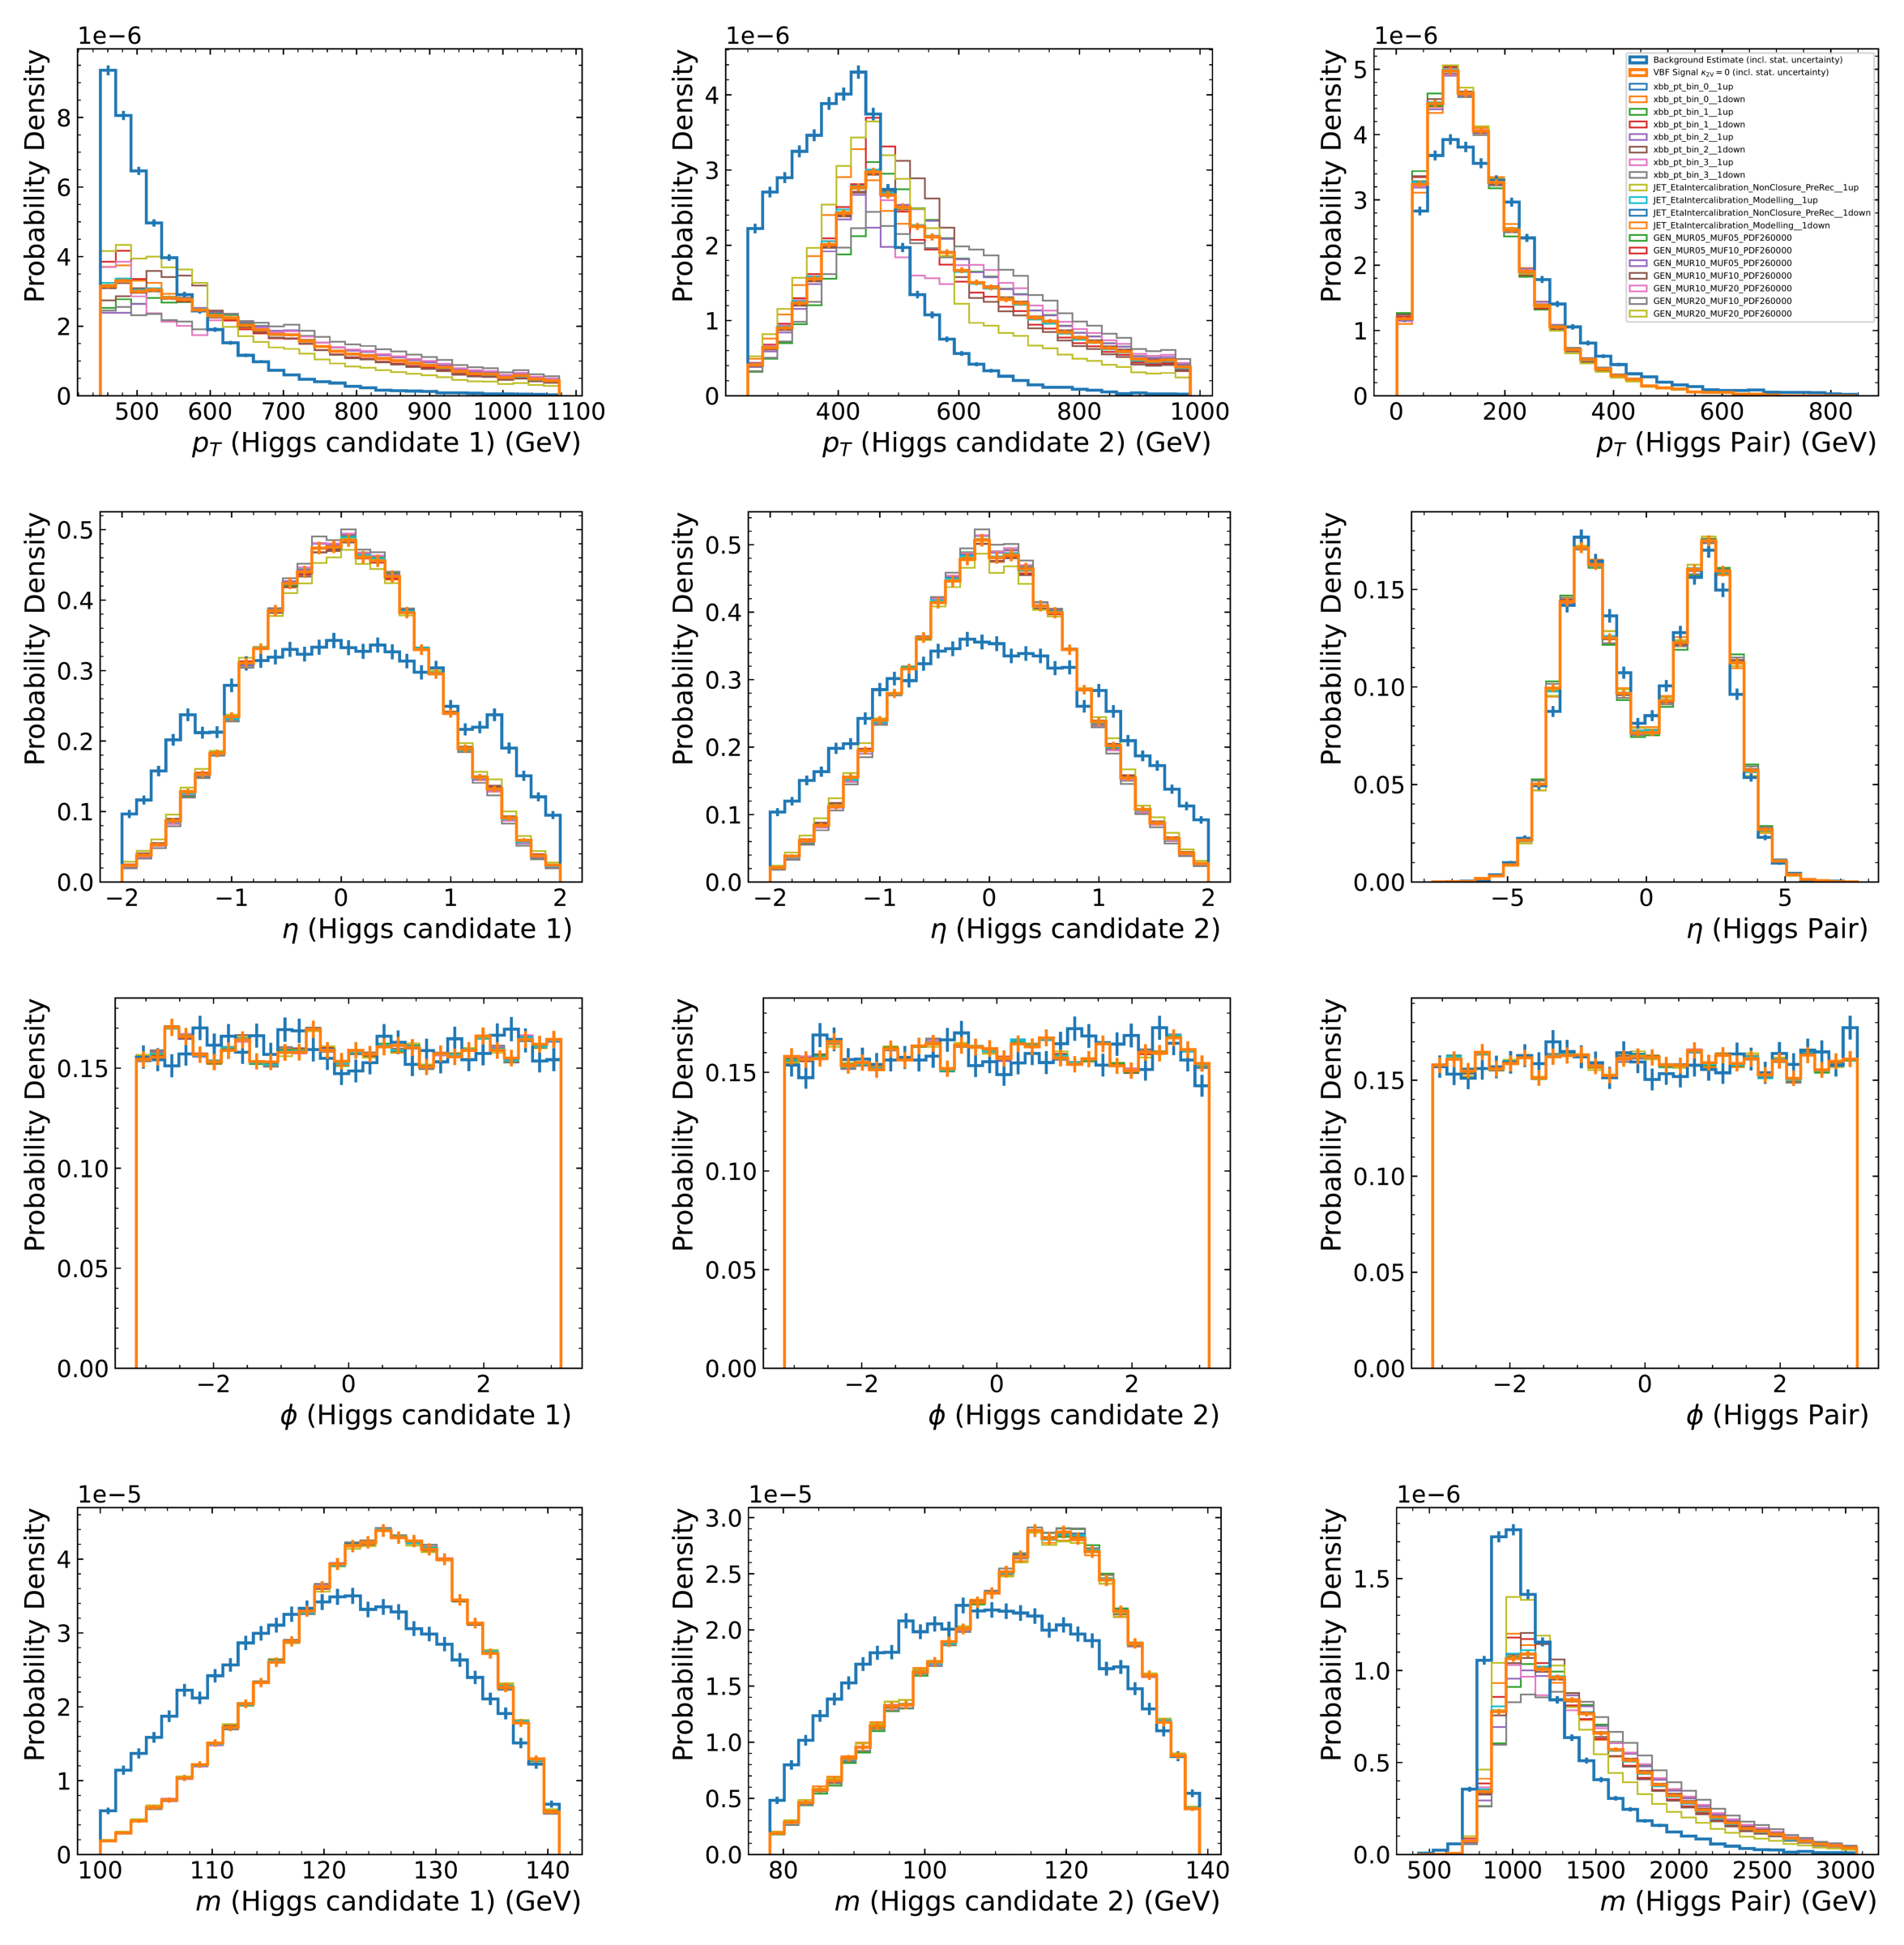
\includegraphics[width=1\textwidth]{neos_results/tomatos_inputs_0}
    \caption[]{Neos input variables (1/2): The coloums from left to right correspond to the four vectors of the leading Higgs candidate, the subleading Higgs candidate and the Higgs Pair system. A legend valid for all figures is shown in the upper right figure.}
    \label{fig:tomatos_inputs_0}
\end{figure}



\begin{figure}
    \centering
    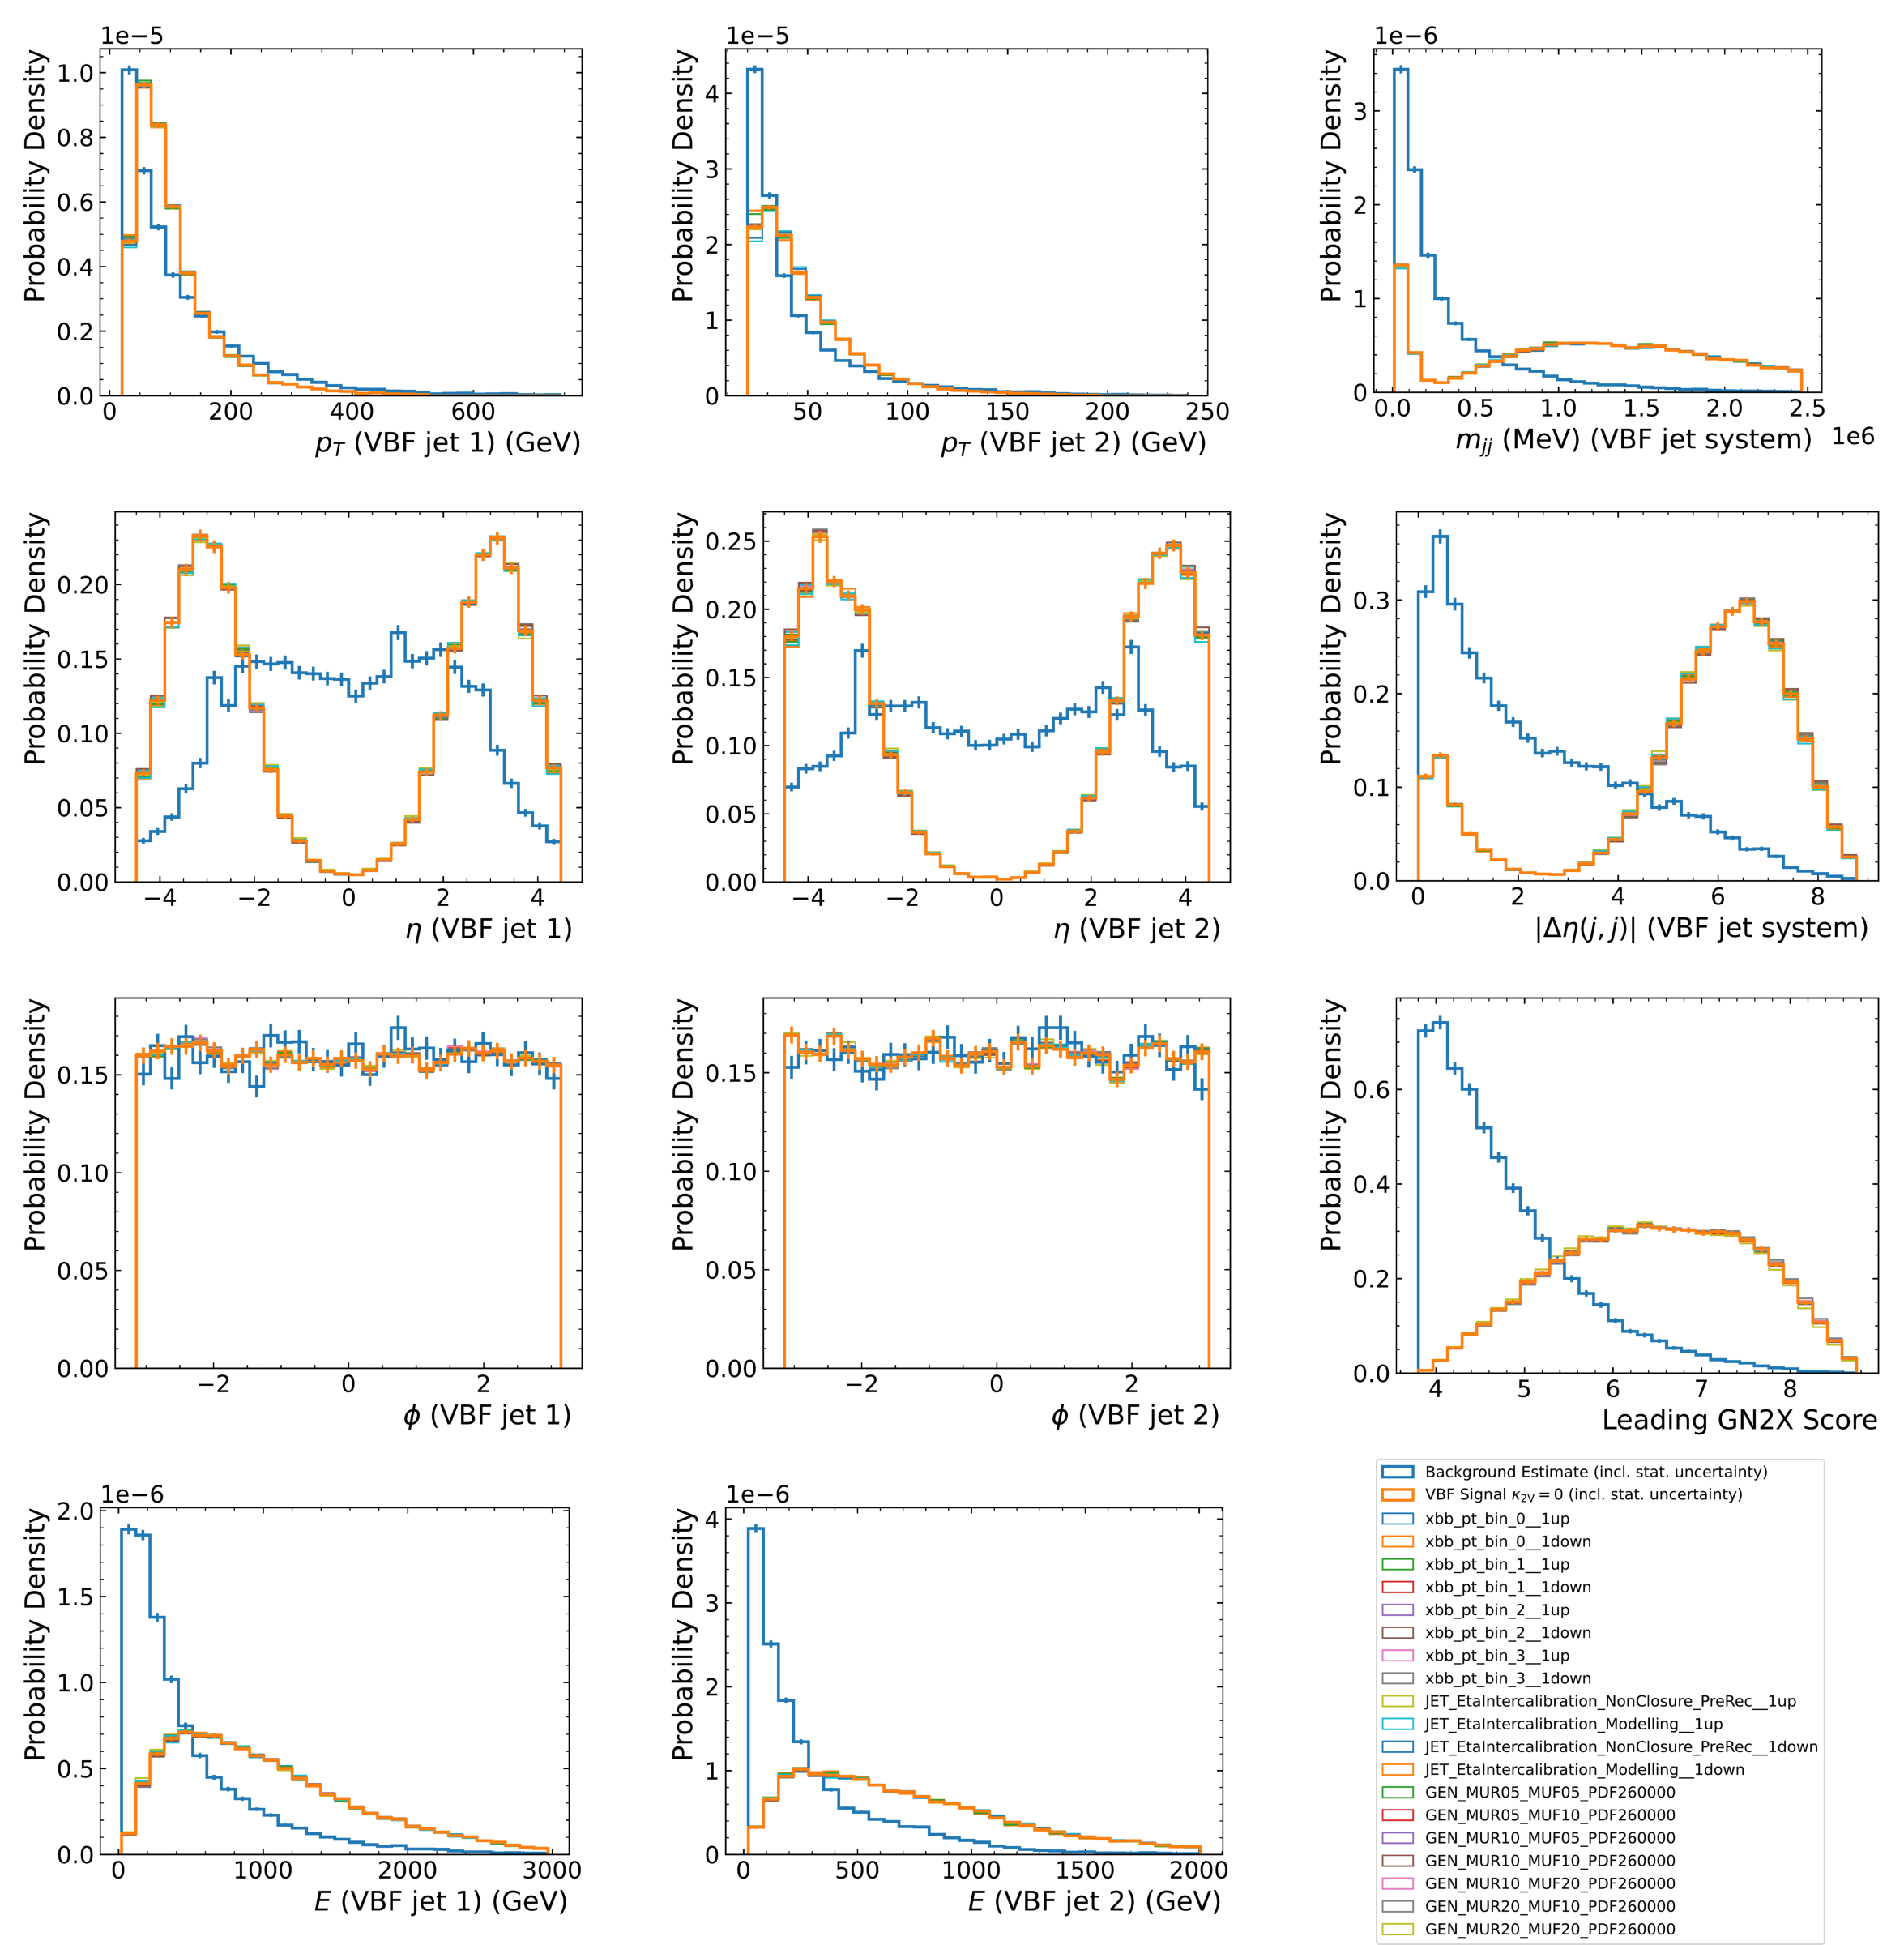
\includegraphics[width=1\textwidth]{neos_results/tomatos_inputs_1}
    \caption[]{Neos input variables (2/2): Columns from left to right: Four vectors of the two vbf jets and the leading GN2X score in the event is depicted above the legend.}
    \label{fig:tomatos_inputs_1}
\end{figure}
